\pdfminorversion=4
\documentclass[aspectratio=169]{beamer}

\mode<presentation>
{
  \usetheme{default}
  \usecolortheme{default}
  \usefonttheme{default}
  \setbeamertemplate{navigation symbols}{}
  \setbeamertemplate{caption}[numbered]
  \setbeamertemplate{footline}[frame number]  % or "page number"
  \setbeamercolor{frametitle}{fg=white}
  \setbeamercolor{footline}{fg=black}
} 

\usepackage[english]{babel}
\usepackage[utf8x]{inputenc}
\usepackage{tikz}
\usepackage{courier}
\usepackage{array}
\usepackage{bold-extra}
\usepackage{minted}
\usepackage[thicklines]{cancel}
\usepackage{fancyvrb}

\xdefinecolor{dianablue}{rgb}{0.18,0.24,0.31}
\xdefinecolor{darkblue}{rgb}{0.1,0.1,0.7}
\xdefinecolor{darkgreen}{rgb}{0,0.5,0}
\xdefinecolor{darkgrey}{rgb}{0.35,0.35,0.35}
\xdefinecolor{darkorange}{rgb}{0.8,0.5,0}
\xdefinecolor{darkred}{rgb}{0.7,0,0}
\definecolor{darkgreen}{rgb}{0,0.6,0}
\definecolor{mauve}{rgb}{0.58,0,0.82}

\title[2019-06-18-cmsml3-uproot]{Uproot: accessing ROOT data in the scientific Python ecosystem}
\author{Jim Pivarski}
\institute{Princeton University -- IRIS-HEP}
\date{June 18, 2019}

\usetikzlibrary{shapes.callouts}

\begin{document}

\logo{\pgfputat{\pgfxy(0.11, 7.4)}{\pgfbox[right,base]{\tikz{\filldraw[fill=dianablue, draw=none] (0 cm, 0 cm) rectangle (50 cm, 1 cm);}\mbox{\hspace{-8 cm}
\includegraphics[height=1 cm]{princeton-logo-long.png}\hspace{0.1 cm}\raisebox{0.1 cm}{
\includegraphics[height=0.8 cm]{iris-hep-logo-long.png}}\hspace{0.1 cm}}}}}

\begin{frame}
  \titlepage
\end{frame}

\logo{\pgfputat{\pgfxy(0.11, 7.4)}{\pgfbox[right,base]{\tikz{\filldraw[fill=dianablue, draw=none] (0 cm, 0 cm) rectangle (50 cm, 1 cm);}\mbox{\hspace{-8 cm}
\includegraphics[height=1 cm]{princeton-logo.png}\hspace{0.1 cm}\raisebox{0.1 cm}{
\includegraphics[height=0.8 cm]{iris-hep-logo.png}}\hspace{0.1 cm}}}}}

% Uncomment these lines for an automatically generated outline.
%\begin{frame}{Outline}
%  \tableofcontents
%\end{frame}

% START START START START START START START START START START START START START

\begin{frame}{Python is the primary interface for machine learning these days}
\vspace{0.5 cm}

\mbox{ } 
\includegraphics[height=0.8 cm]{sklearn-logo.png}
\hfill 
\includegraphics[height=0.8 cm]{pytorch-logo.png}
\hfill 
\includegraphics[height=0.8 cm]{keras-logo.png}
\hfill 
\includegraphics[height=1 cm]{tensorflow-logo.png}
\hfill 
\includegraphics[height=0.8 cm]{caffe2-logo.png}
\hfill 
\includegraphics[height=0.8 cm]{gluon-logo.png} \mbox{ }

\mbox{ } 
\includegraphics[height=0.8 cm]{chainer-logo.png}
\hfill 
\includegraphics[height=1 cm]{cntk-logo.png}
\hfill 
\includegraphics[height=0.8 cm]{lasagne-logo.png}
\hfill 
\includegraphics[height=0.6 cm]{onnx-logo.png}
\hfill 
\includegraphics[height=0.8 cm]{cesium-logo.png}
\hfill 
\includegraphics[height=0.8 cm]{xgboost-logo.png} \mbox{ }

\vspace{1 cm}
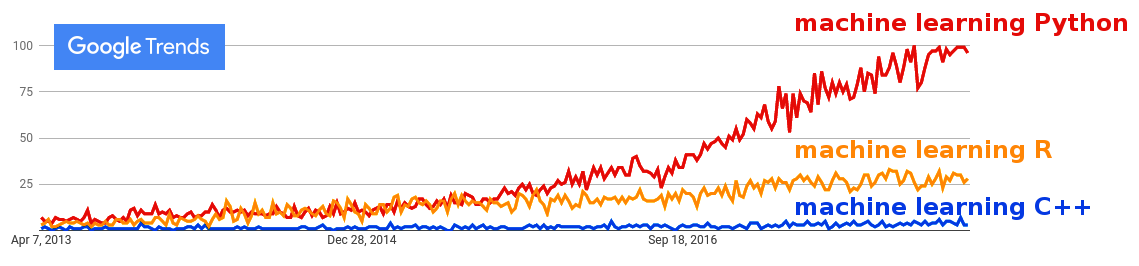
\includegraphics[width=\linewidth]{python-r-cpp-googletrends-machinelearning.png}
\end{frame}

\begin{frame}{ROOT data in Python: three approaches}
\vspace{0.3 cm}
\large
\begin{enumerate}
\item \textcolor{darkblue}{PyROOT:} new methods for direct TTree-to-Numpy translation.
\item \textcolor{darkblue}{root\_numpy:} Python/C++ extension module, compiles into ROOT.
\item \textcolor{darkblue}{uproot:} independent ROOT I/O implementation in Python.
\end{enumerate}

\vspace{0.2 cm}
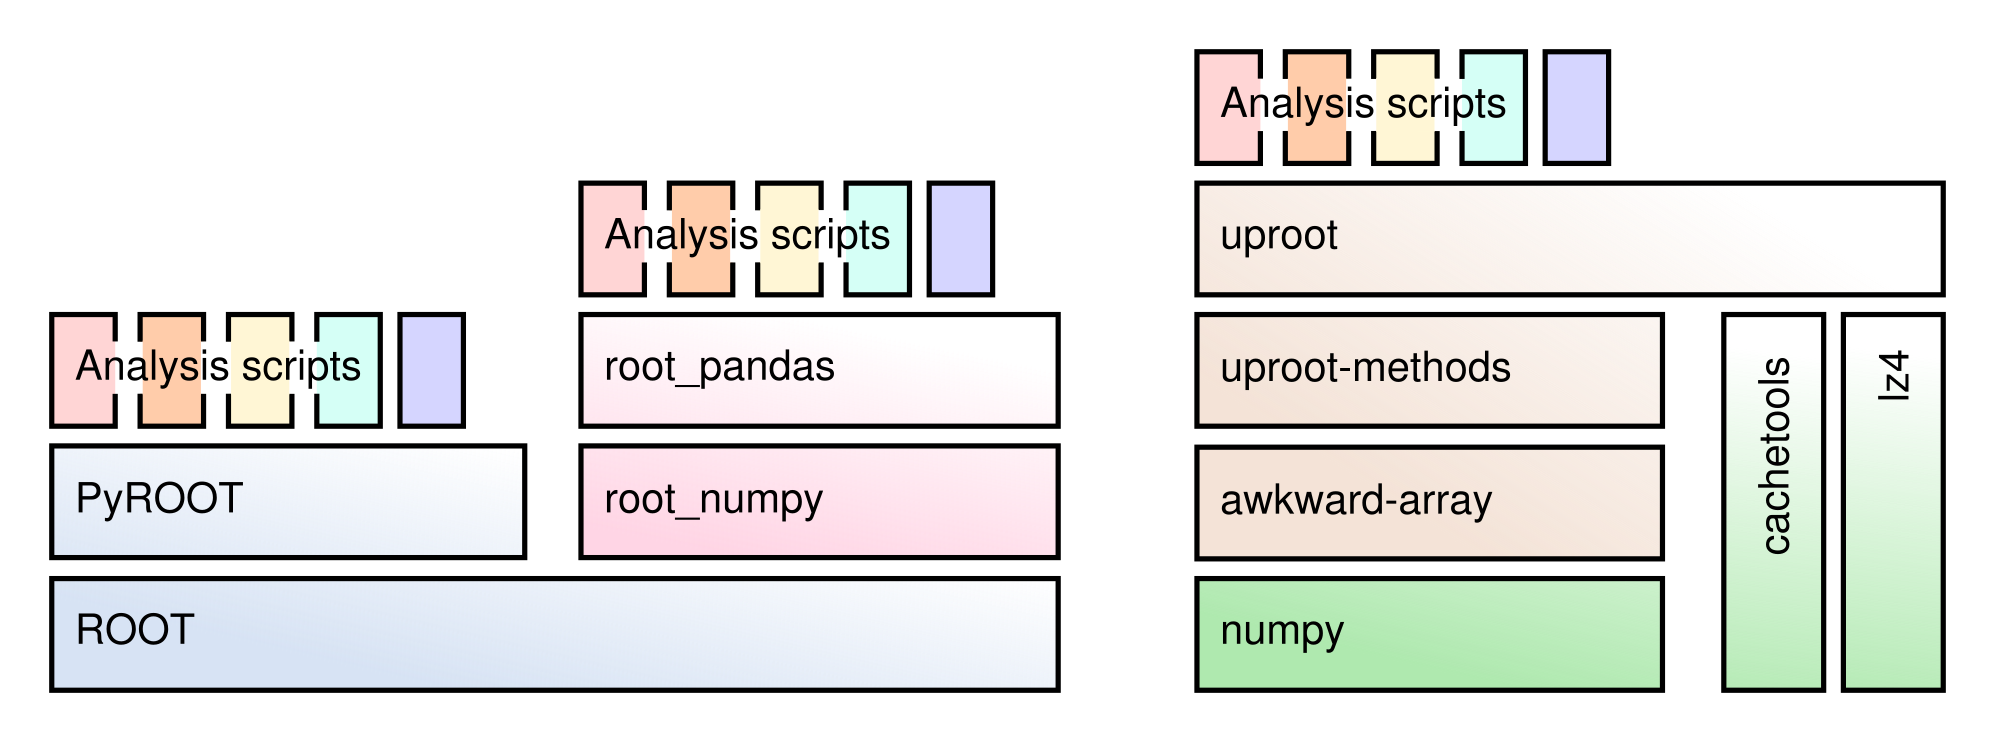
\includegraphics[width=\linewidth]{abstraction-layers.png}
\end{frame}

\begin{frame}{}
\LARGE
\begin{center}
Approach \#1: \textcolor{darkblue}{PyROOT}
\end{center}
\end{frame}

\begin{frame}[fragile]{PyROOT's universal bindings are great, but slow$^2$}
\vspace{0.5 cm}
PyROOT is unique among Python-C++ bindings in that no manual association of Python objects to C++ objects is required (thanks to ROOT/Cling's C++ reflection).

\vspace{0.25 cm}
\small
\begin{minted}{python}
>>> tfile = ROOT.TFile("cms-nanoaod.root")
>>> ttree = tfile.Get("Events")
>>> ttree.SetBranchStatus("*", 0)
>>> ttree.SetBranchStatus("nMuon", 1)
>>> ttree.SetBranchStatus("Muon_pt", 1)
>>> ttree.SetBranchStatus("Muon_eta", 1)

>>> for event in ttree:
...     for pt, eta in zip(event.Muon_pt, event.Muon.eta):
...         pt * math.sinh(eta)
\end{minted}
\large

\vspace{0.25 cm}
BUT the above is \textcolor{darkblue}{$36\times$ slower than pure Python} (and $1000\times$ slower than C++) because of reflection {\it in the loop.}
\end{frame}

\begin{frame}[fragile]{New methods to go directly to Numpy}
\large
\vspace{0.5 cm}
New ``Pythonizations'' are being added to PyROOT for useful features like {\tt AsMatrix}, which fill an array on the C++ side, without reflection.

\small
\begin{minted}{python}
>>> ttree.AsMatrix(["MET_px", "MET_py"])
\end{minted}
\color{darkblue}\vspace{-0.5\baselineskip}\begin{verbatim}
array([[  5.91277122,   2.5636332 ],
       [ 24.76520348, -16.34910965],
       [-25.78508759,  16.23713112],
       ...,
       [ 18.10164642,  50.29071808],
       [ 79.87519073, -52.35145187],
       [ 19.71374893,  -3.59541821]])
\end{verbatim}
\color{black}
\large

\vspace{0.25 cm}
\begin{uncoverenv}<2->
The return type is an unlabeled matrix, but you can ask for the labels explicitly (e.g.\ to make a Pandas DataFrame).

\small
\begin{minted}{python}
data, labels = ttree.AsMatrix(["MET_px", "MET_py"], return_labels=True)
pandas.DataFrame(data, columns=labels)
\end{minted}
\end{uncoverenv}
\end{frame}

\begin{frame}[fragile]{However, {\tt AsMatrix} is only for numeric branches: no collections}
\vspace{0.5 cm}

\small
\begin{minted}{python}
>>> ttree.AsMatrix(["Muon_pt"])  # arbitrary number of muons per event
\end{minted}
\color{darkblue}\vspace{-0.5\baselineskip}\begin{verbatim}
array([[0.],
       [0.],
       [0.],
       ...,
       [0.],
       [0.],
       [0.]])
\end{verbatim}

\vspace{-0.2 cm}
\color{gray}
\begin{verbatim}
Error in <TTreeReaderValueBase::GetBranchDataType()>: Must use
TTreeReaderArray to read branch Muon_pt: it contains an array
or a collection.
\end{verbatim}
\begin{verbatim}
Error in <TTreeReaderValueBase::CreateProxy()>: The branch Muon_pt
contains data of type {UNDETERMINED TYPE}, which does not have a
dictionary.
\end{verbatim}
\end{frame}

\begin{frame}{}
\vspace{-0.1 cm}
\begin{columns}
\column{1.145\linewidth}
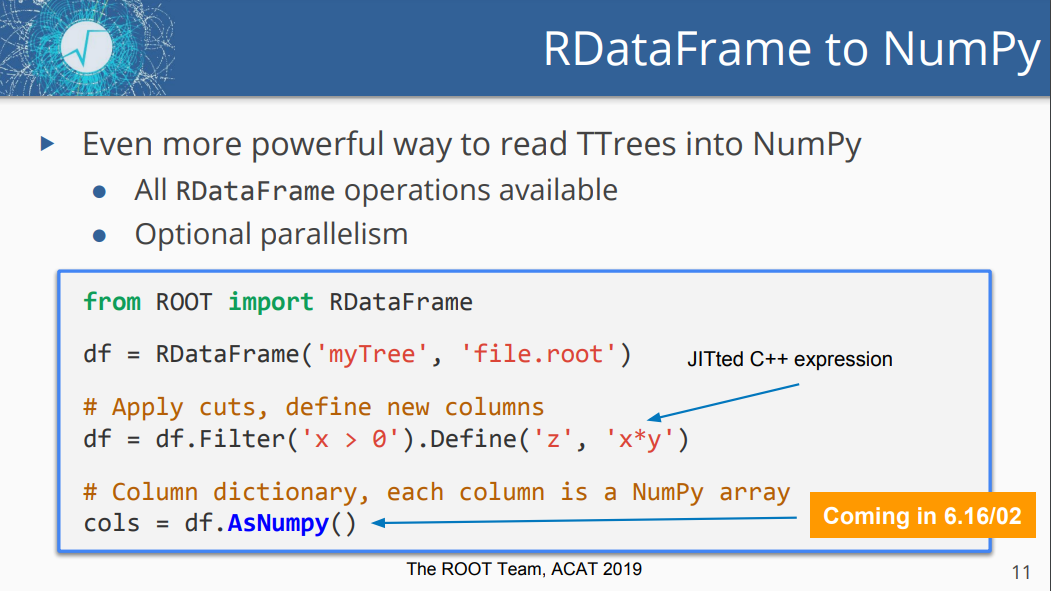
\includegraphics[width=\linewidth]{03-coming-soon-2.png}
\end{columns}
\end{frame}

\begin{frame}{}
\LARGE
\begin{center}
Approach \#2: \textcolor{darkblue}{root\_numpy}
\end{center}
\end{frame}

\begin{frame}[fragile]{root\_numpy compiles into Python and ROOT}
\vspace{0.25 cm}
\small
\begin{minted}{python}
root_numpy.tree2array(ttree, ["MET_px", "MET_py"])    # PyROOT "ttree"

root_numpy.root2array("cms-nanoaod.root", "Events",   # no PyROOT
                      ["MET_px/1000.0", "MET_py/1000.0"])
\end{minted}
\large

\vspace{0.25 cm}
Any {\tt TTree::Draw} expression may be used, not just branch names, and it's as fast as {\tt TTree::Draw}. You can think of it as ``{\tt TTree::Draw} to Numpy.''

\vspace{0.25 cm}
\mbox{ } \hfill 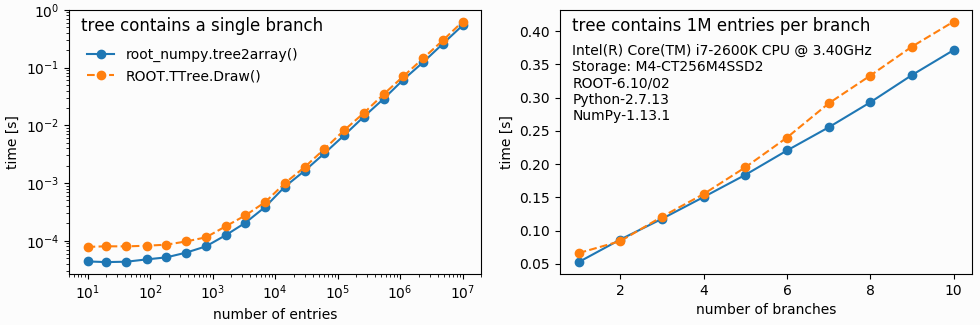
\includegraphics[width=0.8\linewidth]{root-numpy-fast.png} \hfill \mbox{ }
\end{frame}

\begin{frame}[fragile]{Collections in root\_numpy}
\large
\vspace{0.5 cm}

root\_numpy {\it can} read collections of numeric types (``jagged arrays''), but uses the nearest Numpy type: an array whose contents are arrays (i.e. Python objects).

\small
\begin{minted}{python}
>>> root_numpy.tree2array(ttree, "Muon_pt")
\end{minted}
\color{darkblue}\vspace{-\baselineskip}\begin{verbatim}
array([array([], dtype=float32),
       array([], dtype=float32),
       array([5.315762], dtype=float32),
       ...,
       array([26.351288], dtype=float32),
       array([], dtype=float32),
       array([44.28051, 6.6997213], dtype=float32)],
      dtype=object)
\end{verbatim}
\color{black}

\large
Undermines the two advantages of Numpy: speed and flexibility (inner arrays are not recognized as a dimension).
\end{frame}

\begin{frame}{}
\begin{columns}
\column{1.145\linewidth}
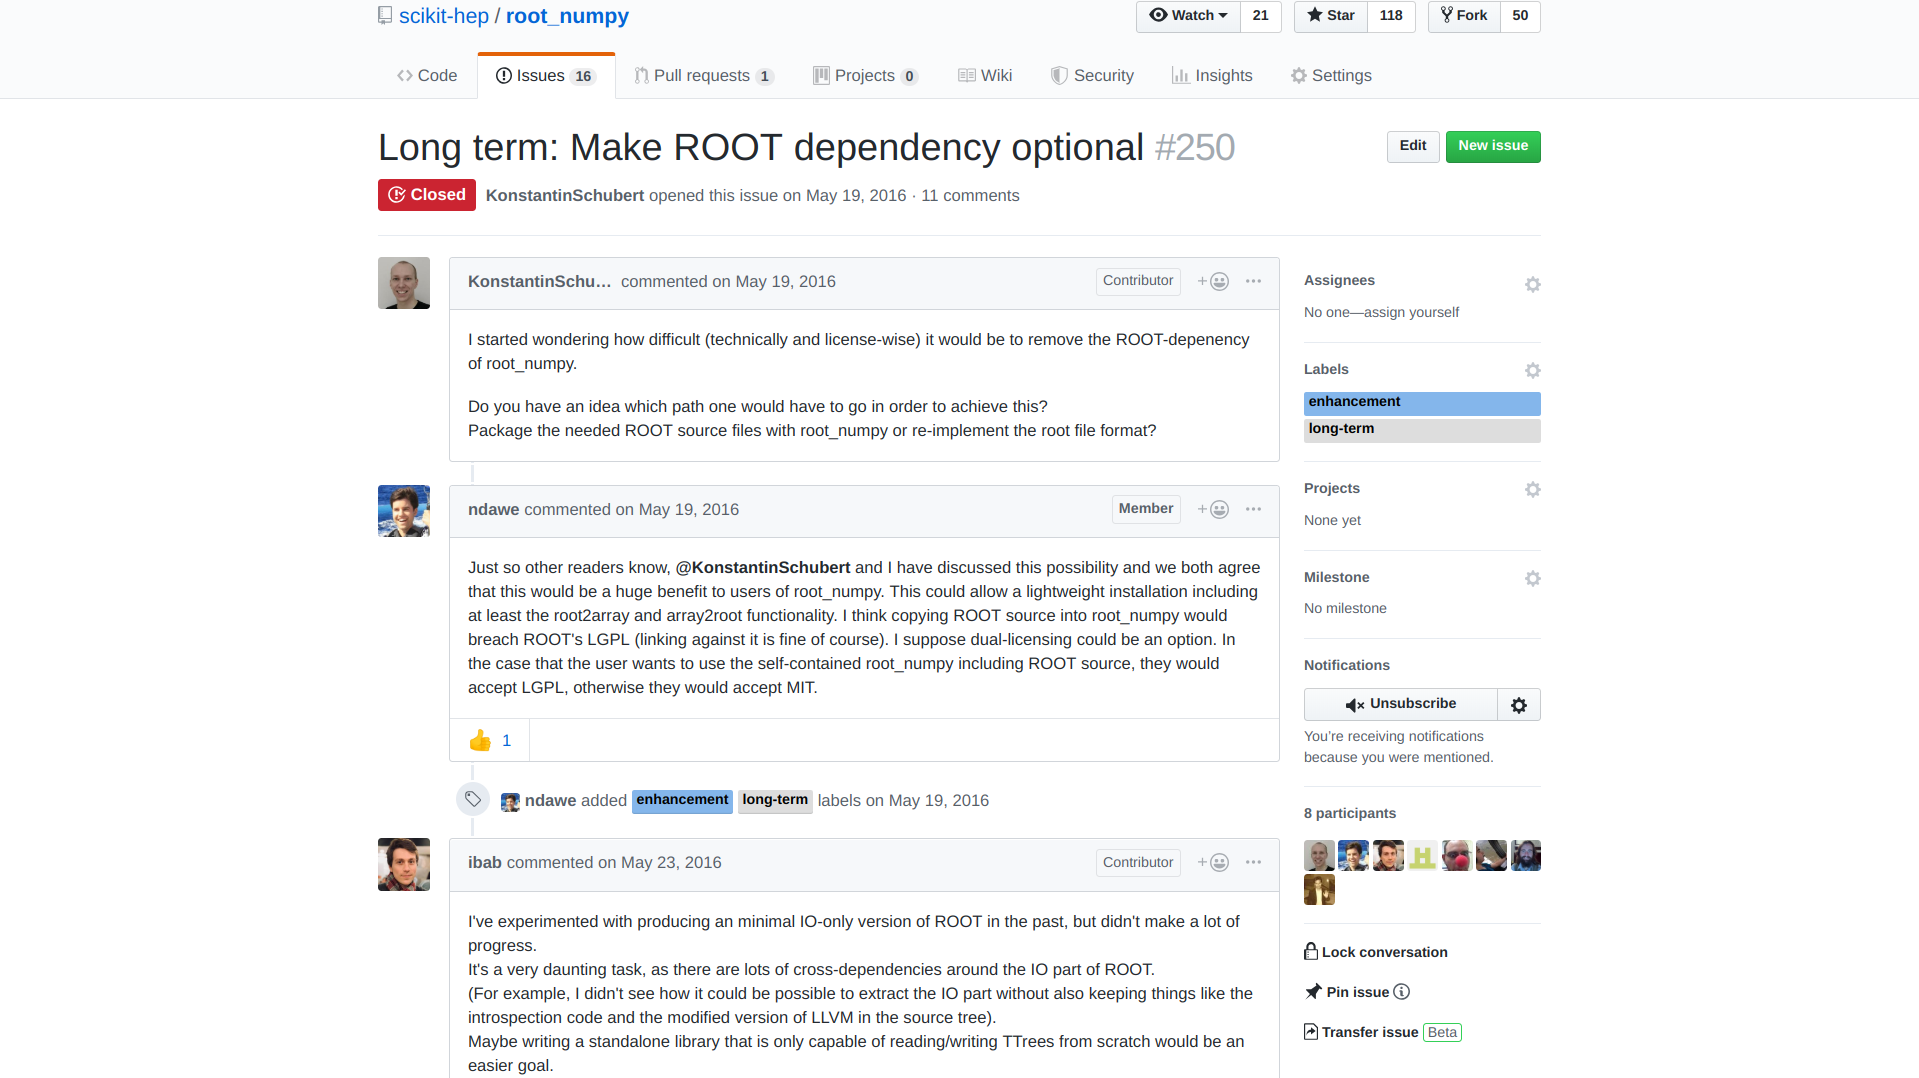
\includegraphics[width=\linewidth]{root-numpy-optionalroot.png}
\end{columns}
\end{frame}

\begin{frame}{}
\LARGE
\begin{center}
Approach \#3: \textcolor{darkblue}{uproot}
\end{center}
\end{frame}

\begin{frame}[fragile]{uproot is a Python reimplementation of ROOT I/O}
\small
\vspace{0.25 cm}

\begin{minted}{python}
uproot.open("cms-nanoaod.root")["Events"].arrays(["MET_px", "MET_py"])
\end{minted}
\color{darkblue}\vspace{-0.5\baselineskip}\begin{verbatim}
{b'MET_px': array([ 5.912771,  24.76520, -25.785088, ...,
                   18.101646,  79.87519,  19.713749], dtype=float32),
 b'MET_py': array([ 2.563633, -16.34911,  16.237131, ...,
                   50.290718, -52.35145,  -3.595418], dtype=float32)}
\end{verbatim}
\color{black}

\large
\begin{uncoverenv}<2->
But it's not slow: it only uses Python to find the baskets and cast \mbox{them as arrays.\hspace{-0.25 cm}} If you have large baskets, that's even better than cycling through events.

\mbox{ } \hfill 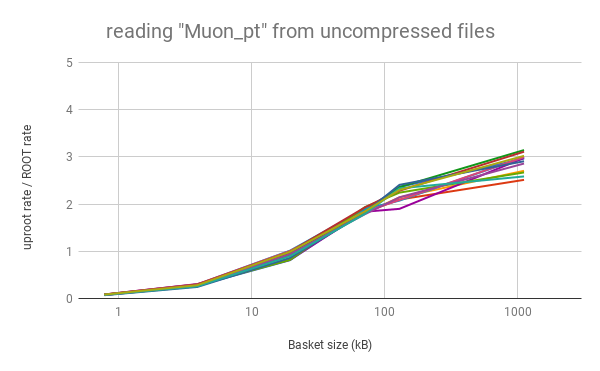
\includegraphics[width=0.45\linewidth]{root-none-muon.png} \hfill 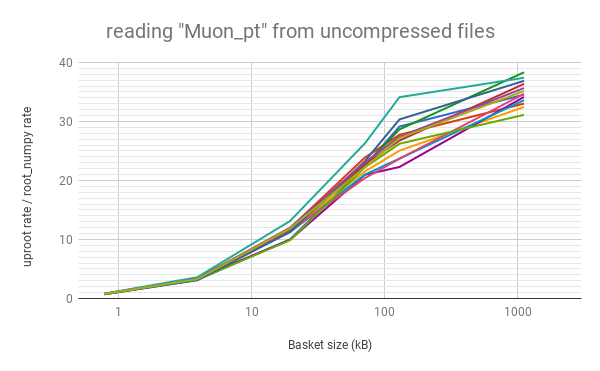
\includegraphics[width=0.45\linewidth]{rootnumpy-none-muon.png} \hfill \mbox{ }
\end{uncoverenv}
\end{frame}

\begin{frame}[fragile]{awkward-array: data structures beyond Numpy}
\large
\vspace{0.25 cm}

Rather than forcing our data structures into Numpy's types, we built new types out of basic arrays.

\begin{columns}
\column{1.07\linewidth}
\small
\begin{minted}{python}
>>> pt = uproot.open("cms-nanoaod.root")["Events"].array("Muon_pt")
>>> pt
\end{minted}

\vspace{-0.6 cm}
\color{darkblue}\begin{verbatim}
<JaggedArray [[] [] [5.315762] ... [26.351288] [] [44.28051 6.6997213]]>
\end{verbatim}
\color{black}

\begin{uncoverenv}<2->
\vspace{-0.6 cm}
\begin{minted}{python}
>>> type(pt)               # not really a Numpy array
\end{minted}

\vspace{-0.6 cm}
\color{darkblue}\begin{verbatim}
<class 'awkward.array.jagged.JaggedArray'>
\end{verbatim}
\color{black}
\end{uncoverenv}

\begin{uncoverenv}<3->
\vspace{-0.6 cm}
\begin{minted}{python}
>>> pt.counts, pt.content  # two contiguous arrays, not millions of them
\end{minted}

\vspace{-0.6 cm}
\color{darkblue}\begin{verbatim}
(array([0, 0, 1, ..., 1, 0, 2]),
 array([5.31576, 47.0548, 19.04261, ..., 26.35128, 44.2805, 6.699721]))
\end{verbatim}
\color{black}
\end{uncoverenv}

\begin{uncoverenv}<4->
\vspace{-0.6 cm}
\begin{minted}{python}
>>> pt[pt.counts > 0]      # filter by elementwise comparison, like Numpy
\end{minted}

\vspace{-0.6 cm}
\color{darkblue}\begin{verbatim}
<JaggedArray [[5.3157] [47.054 19.0426] ... [26.3512] [44.280 6.69972]]>
\end{verbatim}
\color{black}
\end{uncoverenv}

\begin{uncoverenv}<5->
\vspace{-0.6 cm}
\begin{minted}{python}
>>> pt[pt.counts > 0, 0]   # jagged inner data are a slicable dimension
\end{minted}

\vspace{-0.6 cm}
\color{darkblue}\begin{verbatim}
array([5.31576, 47.0548, 15.77672, ..., 10.06197, 26.35128, 44.2805])
\end{verbatim}
\color{black}
\end{uncoverenv}
\end{columns}
\end{frame}

\begin{frame}{Like Numpy itself, awkward operations $\sim$ the speed of C++}
\large
\vspace{0.35 cm}

\textcolor{darkblue}{Very simple benchmark:} \mintinline{python}{pz = pt*numpy.sinh(eta)} for jagged \mintinline{python}{pt}, \mintinline{python}{eta}

\begin{center}
\renewcommand{\arraystretch}{1.25}
\begin{tabular}{c l r}
\hline Python & uproot load $+$ awkward compute & 0.7 + 0.5 = 1.2$\times$ \\
C++ & ROOT TBranch::GetEntry & \phantom{0.7 + 0.5 =} 1$\times$\phantom{.0} \\
C++ & ROOT TTreeReader & \phantom{0.7 + 0.5 =} 2$\times$\phantom{.0} \\
C++ & ROOT RDataFrame & \phantom{0.7 + 0.5 =} 3.5$\times$ \\
Python & root\_numpy load $+$ for loop & 14 + 42 = 56$\times$\phantom{.0} \\
Python & PyROOT & \phantom{0.7 + 0.5 =} 1000$\times$\phantom{.0} \\ \hline
\end{tabular}
\end{center}

\vspace{0.25 cm}
\textcolor{darkblue}{Realistic analysis:} Z mass peak

\vspace{-0.5 cm}
\begin{columns}
\column{0.6\linewidth}
\renewcommand{\arraystretch}{1.25}
\begin{tabular}{c l c r}
\hline Python & uproot $+$ awkward & \href{https://github.com/nsmith-/coffea/blob/master/notebooks/zpeak.ipynb}{\textcolor{blue}{zpeak.ipynb}} & 1.5$\times$ \\
C++ & TBranch::GetEntry & \href{https://github.com/nsmith-/coffea/blob/master/notebooks/ZPeak.C}{\textcolor{blue}{ZPeak.C}} & 1$\times$\phantom{.0} \\ \hline
\end{tabular}

\column{0.25\linewidth}
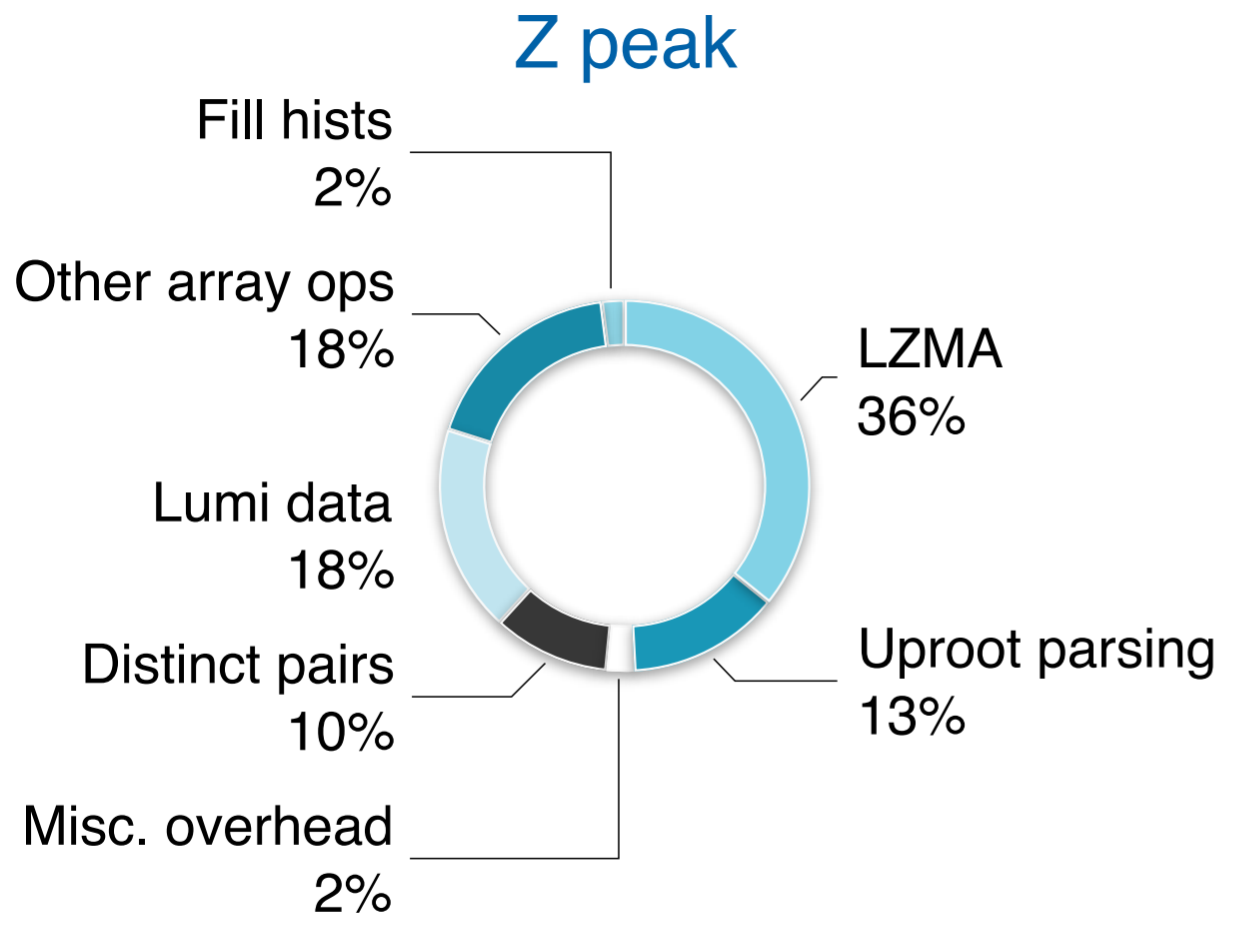
\includegraphics[width=\linewidth]{zpeak-performance-breakdown.png}
\end{columns}
\end{frame}

\begin{frame}[fragile]{Jagged $\to$ flat restructuring: padding and clipping}
\small
\begin{minted}{python}
>>> pt
\end{minted}

\vspace{-0.45 cm}
\color{darkblue}\begin{verbatim}
<JaggedArray [[              ] [         ] [5.315762          ] ...
              [26.351288     ] [         ] [44.28051 6.6997213]]>
\end{verbatim}
\color{black}

\vspace{-0.5\baselineskip}
\begin{minted}{python}
>>> pt.pad(2, clip=True)                        # subarrays → pairs
\end{minted}

\vspace{-0.45 cm}
\color{darkblue}\begin{verbatim}
<JaggedArray [[     None None] [None None] [5.315762 None     ] ...
              [26.351288 None] [None None] [44.28051 6.6997213]]>
\end{verbatim}
\color{black}

\vspace{-0.5\baselineskip}
\begin{minted}{python}
>>> pt.pad(2, clip=True).fillna(0)              # None → 0.0
\end{minted}

\vspace{-0.45 cm}
\color{darkblue}\begin{verbatim}
<JaggedArray [[ 0.0       0.0] [ 0.0  0.0] [5.315762 0.0      ] ...
              [26.351288  0.0] [ 0.0  0.0] [44.28051 6.6997213]]>
\end{verbatim}
\color{black}

\vspace{-0.5\baselineskip}
\begin{minted}{python}
>>> pt.pad(2, clip=True).fillna(0).regular()    # Awkward → Numpy
\end{minted}

\vspace{-0.45 cm}
\color{darkblue}\begin{verbatim}
array([[ 0.        0.       ]
       [ 0.        0.       ]
       [ 5.315762  0.       ]
       ...
       [26.351288  0.       ]
       [ 0.        0.       ]
       [44.28051   6.6997213]])
\end{verbatim}
\color{black}
\end{frame}

\begin{frame}[fragile]{Jagged $\to$ flat restructuring: combinatorics}
\small
\begin{minted}{python}
>>> pairs = pt.choose(2)                         # distinct pairs
>>> pairs
\end{minted}

\vspace{-0.45 cm}
\color{darkblue}\begin{verbatim}
<JaggedArray [[] [] [] ... [] [] [(44.28051, 6.6997213)]]>
\end{verbatim}
\color{black}

\vspace{-0.5\baselineskip}
\begin{minted}{python}
>>> pairs[pairs.counts > 0]                      # drop if no pairs
\end{minted}

\vspace{-0.45 cm}
\color{darkblue}\begin{verbatim}
<JaggedArray [[(47.054, 19.04)]
              [(30.902, 17.22) (30.902, 9.700) (17.228, 9.700)] ...
              [(23.843, 8.940)]
              [(44.280, 6.699)]]>
\end{verbatim}
\color{black}

\vspace{-0.5\baselineskip}
\begin{minted}{python}
>>> pairs[pairs.counts > 0].flatten().unzip()    # split left-right
\end{minted}

\vspace{-0.45 cm}
\color{darkblue}\begin{verbatim}
(array([47.0548, 30.9022, 30.9022, ..., 36.5802, 23.8430, 44.2805]),
 array([19.0426, 17.2284,  9.7000, ...,  9.5405,  8.9407 , 6.6997]))
\end{verbatim}
\color{black}

\vspace{-0.5\baselineskip}
\begin{minted}{python}
>>> numpy.stack(pairs[pairs.counts > 0].flatten().unzip(), axis=1)
\end{minted}

\vspace{-0.45 cm}
\color{darkblue}\begin{verbatim}
array([[47.05483  19.042616]
       [30.902279 17.228409]
       ...,
       [23.843002  8.940705]
       [44.28051   6.6997213]])
\end{verbatim}
\color{black}
\end{frame}

\begin{frame}[fragile]{Pandas DataFrames}
\small
\begin{minted}{python}
>>> ttree.pandas.df(["MET_pt", "MET_phi", "Muon_pt", "Muon_phi"],
                    flatten=False)     # jaggedness → Python lists
\end{minted}
\scriptsize\color{darkblue}\vspace{-0.75\baselineskip}\begin{verbatim}
                     MET_pt   MET_phi                Muon_pt                 Muon_phi
entry                                                                                
0                 38.405140 -1.961670                     []                       []
1                 49.339661  0.993286                     []                       []
2                 42.162205 -0.966919             [5.315762]              [2.6958008]
3                119.623192  2.034668  [47.05483, 19.042616] [-2.1259766, -2.4106445]
4                 86.078926 -1.925293            [15.776729]              [-1.373291]
5                 45.805889 -0.627319            [14.511511]              [3.0561523]
6                 28.122215 -2.456543                     []                       []
7                105.373856 -0.229370             [68.83148]            [0.044891357]
...                     ...       ...                    ...                      ...
499993           216.192505 -1.008545            [38.096928]             [-2.6450195]
499994           315.657074  2.213867             [36.54806]             [0.86608887]
499995            71.399872  1.185547            [10.061976]             [-2.0263672]
499996            71.563873  0.657593                     []                       []
499997           166.024155  1.468506            [26.351288]              [0.7145996]
499998           115.803070  1.896973                     []                       []
499999            36.379166  1.241699  [44.28051, 6.6997213] [2.383789, -0.070617676]

[500000 rows x 5 columns]
\end{verbatim}
\end{frame}

\begin{frame}[fragile]{Pandas DataFrames}
\small
\begin{minted}{python}
>>> ttree.pandas.df(["MET_pt", "MET_phi", "Muon_pt", "Muon_phi"],
                    flatten=True)      # jaggedness → MultiIndex
\end{minted}
\scriptsize\color{darkblue}\vspace{-0.75\baselineskip}\begin{verbatim}
                     MET_pt   MET_phi                Muon_pt                 Muon_phi
entry  subentry                                                      
2      0          42.162205 -0.966919               5.315762                 2.695801
3      0         119.623192  2.034668              47.054829                -2.125977
       1         119.623192  2.034668              19.042616                -2.410645
4      0          86.078926 -1.925293              15.776729                -1.373291
5      0          45.805889 -0.627319              14.511511                 3.056152
7      0         105.373856 -0.229370              68.831482                 0.044891
8      0          79.144371 -0.178497              30.902279                 1.756836
       1          79.144371 -0.178497              17.228409                -2.797363
...                     ...       ...                    ...                      ...
499992 0          42.763760 -2.555664              23.843002                -1.728516
       1          42.763760 -2.555664               8.940705                -0.108810
499993 0         216.192505 -1.008545              38.096928                -2.645020
499994 0         315.657074  2.213867              36.548061                 0.866089
499995 0          71.399872  1.185547              10.061976                -2.026367
499997 0         166.024155  1.468506              26.351288                 0.714600
499999 0          36.379166  1.241699              44.280510                 2.383789
       1          36.379166  1.241699               6.699721                -0.070618
[537189 rows x 4 columns]
\end{verbatim}
\end{frame}

\begin{frame}[fragile]{Pandas DataFrames}
\large
\vspace{0.25 cm}

New method (experimental): make Pandas recognize jagged arrays as columns.

\small
\begin{minted}{python}
>>> ttree.array("Muon_pt").pandas    # JaggedArray → JaggedSeries
\end{minted}
\scriptsize\color{darkblue}\vspace{-0.75\baselineskip}\begin{Verbatim}[commandchars=\\\{\}]
<\textcolor{darkorange}{\textbf{JaggedSeries}} [[] [] [5.315762] ... [26.351288] [] [44.28051 6.6997213]]>
\end{Verbatim}
\color{black}

\small
\begin{minted}{python}
>>> pandas.Series(ttree.array("Muon_pt").pandas)
\end{minted}
\scriptsize\color{darkblue}\vspace{-0.75\baselineskip}\begin{Verbatim}[commandchars=\\\{\}]
0                                      []
1                                      []
2                              [5.315762]
3                   [47.05483  19.042616]
4                             [15.776729]
5                             [14.511511]
6                                      []
                       ...               
499994                         [36.54806]
499995                        [10.061976]
499996                                 []
499997                        [26.351288]
499998                                 []
499999            [44.28051    6.6997213]
Length: 500000, \textcolor{darkorange}{\textbf{dtype: awkward}}
\end{Verbatim}
\color{black}
\large

\vspace{-3 cm}
\hfill \begin{minipage}{0.35\linewidth}
Thanks to Michael Hedges!
\end{minipage}
\vspace{3 cm}
\end{frame}

\begin{frame}{Three ways to get data}
\vspace{0.5 cm}
\begin{columns}
\column{1.05\linewidth}

\renewcommand{\arraystretch}{1.5}
\begin{tabular}{p{0.29\linewidth} c p{0.29\linewidth} c p{0.31\linewidth}}
{\LARGE\bf Direct} & & {\LARGE\bf Lazy} & & {\LARGE\bf Iterative} \\
Simply read from the file and return an array. & & Get an object that reads on demand; transparently work on big data. & & Read arrays in batches for more control over loading and unloading of data. \\
\begin{minipage}{\linewidth}
\vspace{0.5\baselineskip}
\begin{itemize}
\item \href{https://uproot.readthedocs.io/en/latest/ttree-handling.html\#id11}{\textcolor{blue}{TBranch.array}}
\item \href{https://uproot.readthedocs.io/en/latest/ttree-handling.html\#array}{\textcolor{blue}{TTree.array}}
\item \href{https://uproot.readthedocs.io/en/latest/ttree-handling.html\#arrays}{\textcolor{blue}{TTree.arrays}}
\end{itemize}
\vspace{2\baselineskip}
\end{minipage} & &
\begin{minipage}{\linewidth}
\vspace{0.5\baselineskip}
\begin{itemize}
\item \href{https://uproot.readthedocs.io/en/latest/ttree-handling.html\#id13}{\textcolor{blue}{TBranch.lazyarray}}
\item \href{https://uproot.readthedocs.io/en/latest/ttree-handling.html\#lazyarray}{\textcolor{blue}{TTree.lazyarray}}
\item \href{https://uproot.readthedocs.io/en/latest/ttree-handling.html\#lazyarrays}{\textcolor{blue}{TTree.lazyarrays}}
\item \href{https://uproot.readthedocs.io/en/latest/opening-files.html\#uproot-lazyarray-and-lazyarrays}{\textcolor{blue}{uproot.lazyarray}}*
\item \href{https://uproot.readthedocs.io/en/latest/opening-files.html\#uproot-lazyarray-and-lazyarrays}{\textcolor{blue}{uproot.lazyarrays}}*
\end{itemize}
\end{minipage} & &
\begin{minipage}{\linewidth}
\vspace{0.5\baselineskip}
\begin{itemize}
\item \href{https://uproot.readthedocs.io/en/latest/ttree-handling.html\#iterate}{\textcolor{blue}{TTree.iterate}}
\item \href{https://uproot.readthedocs.io/en/latest/opening-files.html\#uproot-iterate}{\textcolor{blue}{uproot.iterate}}*
\item \href{https://uproot.readthedocs.io/en/latest/opening-files.html\#uproot-pandas-iterate}{\textcolor{blue}{uproot.pandas.iterate}}*
\vspace{2.7\baselineskip}
\end{itemize}
\end{minipage}
\end{tabular}
\end{columns}

\vspace{0.5 cm}
*Lazy arrays/iteration over sets of files.
\end{frame}

\begin{frame}[fragile]{Direct $\to$ iterative}
\large
\vspace{0.25 cm}
If you have a small file, you can simply read the whole thing into arrays.

\small
\begin{minted}{python}
pt, eta = ttree.arrays(["Muon_pt", "Muon_eta"], outputtype=tuple)
pz = pt * numpy.sinh(eta)        # calculate everything at once

counts, edges = numpy.histogram(pz.flatten(),
                    bins=100, range=(-2000, 2000))
\end{minted}

\large
\vspace{-0.1 cm}
\begin{uncoverenv}<2->
but if you have many files or limited memory, iterate over chunks.

\small
\vspace{-0.1 cm}
\begin{minted}{python}
counts = None
for pt, eta in uproot.iterate("cms-nanoaod/*.root", "Events",
        ["Muon_pt", "Muon_eta"], outputtype=tuple, entrysteps="3 GB"):
    pz = pt * numpy.sinh(eta)    # calculate 3 GB at a time
    newcounts, edges = numpy.histogram(pz.flatten(),
                           bins=100, range=(-2000, 2000))
    if counts is None:
        counts = newcounts
    else:
        counts += newcounts
\end{minted}
\large

\vspace{-1.3 cm}
\hfill \begin{minipage}{0.35\linewidth}
Same array calculation (\mintinline{python}{pz}), but merging is manual.
\end{minipage}
\vspace{1.3 cm}
\end{uncoverenv}
\end{frame}

\begin{frame}[fragile]{Direct $\to$ lazy}
\large
\vspace{0.25 cm}

The good thing about direct $\to$ iterative is that your array-processing code doesn't have to change (they're just smaller arrays).

\vspace{0.25 cm}
The bad thing is that it has to be embedded in an explicit loop.

\vspace{0.25 cm}
\begin{uncoverenv}<2->
Lazy arrays have an interface like direct arrays but internally iterate in chunks.

\small
\begin{minted}{python}
>>> ttree.array("Muon_pt")      # loads whole array, contiguously
\end{minted}

\vspace{-0.4 cm}
\color{darkblue}\begin{verbatim}
<JaggedArray  [[] [] [5.31576] ... [26.35128] [] [44.2805 6.699721]]>
\end{verbatim}
\color{black}

\vspace{-0.4 cm}
\begin{minted}{python}
>>> ttree.lazyarray("Muon_pt")  # loads first and last chunk (to print)
\end{minted}

\vspace{-0.4 cm}
\color{darkblue}\begin{verbatim}
<ChunkedArray [[] [] [5.31576] ... [26.35128] [] [44.2805 6.699721]]>
\end{verbatim}
\color{black}\large
\end{uncoverenv}

\begin{uncoverenv}<3->
The following splits data into 1~GB chunks, loading no more than 3~GB at a time, and computes \mintinline{python}{pz} from \mintinline{python}{Muon_pt} and \mintinline{python}{Muon_eta}.

\small
\begin{minted}{python}
>>> cache = uproot.ArrayCache("3 GB")
>>> events = uproot.lazyarrays("cms-nanoaod/*.root", "Events",
                               entrysteps="1 GB", cache=cache)
>>> pz = events.Muon_pt * numpy.sinh(events.Muon_eta)
\end{minted}
\end{uncoverenv}
\end{frame}

\begin{frame}[fragile]{Lazy profile: CMS NanoAOD}
\large
\vspace{0.5 cm}

\begin{columns}
\column{1.05\linewidth}
If you know your TTrees are CMS NanoAOD, you can get lazy arrays restructured in an event hierarchy:

\small
\begin{minted}{python}
>>> events = ttree.lazyarrays(profile="cms.nanoaod")
>>> events
\end{minted}

\vspace{-0.6 cm}
\color{darkblue}\begin{verbatim}
<Table [<Event 0> <Event 1> ... <Event 499998> <Event 499999>]>
\end{verbatim}
\color{black}

\vspace{-0.6 cm}
\begin{minted}{python}
>>> events.muons        # now it reads nMuon...
\end{minted}

\vspace{-0.6 cm}
\color{darkblue}\begin{verbatim}
<ChunkedArray [[] [] [<Muon 0>] ... [] [<Muon 537187> <Muon 537188>]]>
\end{verbatim}
\color{black}

\vspace{-0.6 cm}
\begin{minted}{python}
>>> events.muons.pt     # now it reads Muon_pt...
\end{minted}

\vspace{-0.6 cm}
\color{darkblue}\begin{verbatim}
<ChunkedArray [[] [] [5.315762] ... [] [44.28051 6.6997213]]>
\end{verbatim}
\color{black}

\vspace{-0.6 cm}
\begin{minted}{python}
>>> events.columns      # to see structure (also tab-complete)
\end{minted}

\vspace{-0.6 cm}
\color{darkblue}\begin{verbatim}
['run', 'lumi', 'event', 'electrons', 'muons', 'taus', 'photons',
 'jets', 'fatjets', 'subjets', 'isotracks', 'softjets', 'softactivity',
 'fixedGridRhoFastjet', 'MET', 'rawMET', 'caloMET', 'puppiMET', 'tkMET',
 'PV', 'SVs', 'otherPVs', 'pileup', 'trigobjs', 'gen', 'etc', 'raw']
\end{verbatim}
\color{black}
\end{columns}
\end{frame}

\begin{frame}[fragile]{Lazy profile: CMS NanoAOD}
\large
\vspace{0.3 cm}

Since everything is loaded on demand, some fields can be defined in terms of others without unnecessary reading or memory use.

\small
\begin{minted}{python}
>>> events.muons.p4     # now it reads Muon_eta, Muon_phi, Muon_mass
\end{minted}

\vspace{-0.4 cm}
\color{darkblue}\begin{verbatim}
<ChunkedArray [[] []
               [TLorentzVector(5.315, 1.127, 2.695, 0.1057)]
               ...
               [TLorentzVector(44.281, 0.7856,  2.3838, 0.10571)
                TLorentzVector(6.6997, 1.9197, -0.0706, 0.10571)]]>
\end{verbatim}
\color{black}\large

\begin{uncoverenv}<2->
Cross-references are presented as objects, too.

\small
\begin{minted}{python}
>>> events.muons.jet    # now it reads Muon_JetIdx and nJet
\end{minted}

\vspace{-0.3 cm}
\color{darkblue}\begin{verbatim}
<ChunkedArray [[] [] [<Jet 12>] ... [<Jet 4102602> <Jet 4102603>]]>
\end{verbatim}
\color{black}\large
\end{uncoverenv}

\begin{uncoverenv}<3->
So we can compute things like ``$\Delta \phi$ between every muon and its associated jet.''

\small
\begin{minted}{python}
>>> events.muons.p4.delta_phi(events.muons.jet.p4)
\end{minted}

\vspace{-0.3 cm}
\color{darkblue}\begin{verbatim}
<ChunkedArray [[] [] [-0.118652344] ... [0.0009765625 0.1444397]]>
\end{verbatim}
\color{black}
\end{uncoverenv}
\end{frame}

\begin{frame}{With lazy arrays, uproot now uses half of the awkward-array classes}
\vspace{0.35 cm}
\begin{columns}
\column{1.1\linewidth}
\begin{tabular}{p{0.26\linewidth} p{0.71\linewidth}}
\textcolor{mauve}{\mintinline{python}{JaggedArray}}        & \textcolor{mauve}{array containing variable-length subarrays} \\
\textcolor{red}{\mintinline{python}{Table}}                & \textcolor{red}{struct of arrays, presented as an array of structs} \\
\textcolor{red}{\mintinline{python}{ObjectArray}}          & \textcolor{red}{creates Python objects on demand, such as \mintinline{python}{TLorentzVector}} \\
\textcolor{red}{\mintinline{python}{Methods}}              & \textcolor{red}{vectorized methods, like \mintinline{python}{muons.delta_phi(muons.jet)}} \\
\textcolor{blue}{\mintinline{python}{StringArray}}         & \textcolor{blue}{strings (jagged array of characters)} \\
\mintinline{python}{IndexedArray}                          & ``pointers'' into another array (via integer indexes) \\
\mintinline{python}{SparseArray}                           & inverse of {\tt IndexedArray}: zero everywhere except specified indexes \\
\mintinline{python}{MaskedArray}                           & marks elements as {\tt None} with a byte array \\
\textcolor{blue}{\mintinline{python}{BitMaskedArray}}      & \textcolor{blue}{marks elements as {\tt None} with a bit array} \\
\textcolor{red}{\mintinline{python}{IndexedMaskedArray}}   & \textcolor{red}{indexes and masks in one array to avoid placeholders in the data array} \\
\mintinline{python}{UnionArray}                            & contains multiple (enumerated) types \\
\textcolor{mauve}{\mintinline{python}{ChunkedArray}}       & \textcolor{mauve}{view discontiguous memory buffers as one array} \\
\mintinline{python}{AppendableArray}                       & efficiently grow an array in chunks \\
\textcolor{mauve}{\mintinline{python}{VirtualArray}}       & \textcolor{mauve}{load data on demand} \\
\end{tabular}

\vspace{-0.25 cm}
\begin{center}
\begin{minipage}{0.63\linewidth}
\small
\textcolor{red}{used by uproot to read ROOT}, \textcolor{blue}{used to read Parquet}, \textcolor{mauve}{used for both}

lazy arrays are \mintinline{python}{ChunkedArrays} containing \mintinline{python}{VirtualArrays}.
\end{minipage}
\end{center}
\end{columns}
\end{frame}

\begin{frame}{Conclusions}
\Large
\vspace{0.25 cm}

\begin{itemize}\setlength{\itemsep}{0.2 cm}
\item PyROOT's interoperability with Numpy is improving: \mintinline{c++}{TTree::AsMatrix} and \mintinline{c++}{RDataFrame::AsNumpy}.
\item PyROOT's \mintinline{c++}{AsMatrix} and root\_numpy both have issues with jagged array structures.
\item uproot built on awkward-array, which extends Numpy's data structures, including operations to deal with particle kinematics.
\item Try the awkward-array Pandas extension by Michael Hedges.
\item New lazy array methods in uproot to simplify handling of big or multi-file arrays.
\item NanoAOD profile gives a high-level interface to CMS data.
\end{itemize}
\end{frame}

\end{document}
